\subsubsection{UC15 - Gestione IVA}
\begin{figure}[H]
	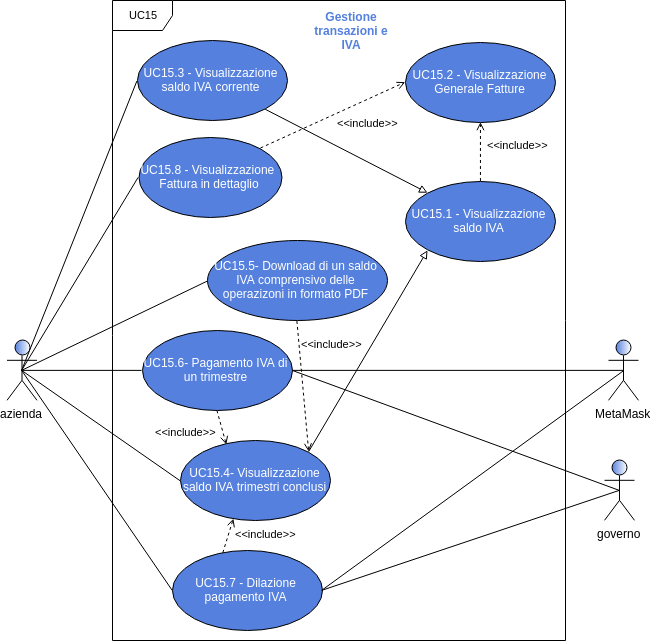
\includegraphics[width=8cm]{res/images/UC15-Generale.png}
	\centering
	\caption{UC15 - Operazioni riguardanti la gestione dell'IVA}
\end{figure}
\begin{itemize}
	\item \textbf{Attori Primari}: azienda;
	\item \textbf{Descrizione}: alle aziende sono messe a disposizione diverse operazioni per gestire l'IVA, come la visualizzazione dei saldi IVA riguardanti diversi trimestri, il download delle informazioni relative ad un trimestre IVA, ed il pagamento dell'IVA a debito al governo\glo, relativa ad un trimestre;
	\item \textbf{Scenario principale}: l'utente visualizza e svolge alcune operazioni per gestire l'IVA;
	\item \textbf{Precondizione}: il sistema ha riconosciuto l'utente autenticato come azienda, e mette a disposizione tutte le pagine necessarie alla visualizzazione e gestione dell'IVA;
	\item \textbf{Postcondizione}: l'azienda ha visualizzato e/o svolto delle operazioni riguardanti l'IVA.
\end{itemize} 
\subsubsection{UC15.1 - Visualizzazione saldo IVA corrente}
\begin{itemize}
	\item \textbf{Attori Primari}: azienda;
	\item \textbf{Descrizione}: l'azienda può visualizzare il saldo parziale relativo al trimestre corrente;
	\item \textbf{Scenario principale}: l'utente visualizza il saldo parziale relativo al trimestre corrente;
	\item \textbf{Precondizione}: il sistema ha riconosciuto l'utente autenticato come azienda, e mette a disposizione le pagine per la gestione dell'IVA. L'utente ha acceduto alla pagina principale per la gestione dell'IVA; 
	\item \textbf{Postcondizione}: l'azienda ha visualizzato il saldo IVA parziale riguardante il trimestre corrente ed è a conoscenza dall'attuale situazione di debito o credito verso il governo.
\end{itemize} 

\subsubsection{UC15.2 - Visualizzazione saldo IVA trimestri conclusi}
\begin{itemize}
	\item \textbf{Attori Primari}: azienda;
	\item \textbf{Descrizione}: l'azienda può visualizzare la lista dei saldi IVA relativi ai trimestri già conclusi. Può inoltre leggere il loro stato, ovvero sapere se i pagamenti a debito o credito con il governo sono saldati oppure no. In caso di stato di debito relativo ad un trimestre, è resa disponibile la possibilità di effettuare il pagamento;
	\item \textbf{Scenario principale}: l'utente visualizza la lista dei saldi IVA dei trimestri passati e per ognuno di essi ottiene l'informazione sullo stato del pagamento dell'IVA, assieme alle operazioni che possono essere effettuate su di esse;
	\item \textbf{Precondizione}: il sistema ha riconosciuto l'utente autenticato come azienda, e mette a disposizione le pagine per la gestione dell'IVA. L'utente ha espresso la volontà di visualizzare la lista dei saldi IVA dei trimestri conclusi;
	\item \textbf{Postcondizione}: l'azienda ha visualizzato il saldo IVA riguardante i trimestri conclusi. Per ognuno di esso ha visualizzato le possibili operazioni da effettuare.
\end{itemize} 
\subsubsection{UC15.3 - Visualizzazione operazioni relative saldo IVA trimestri conclusi}
\begin{itemize}
	\item \textbf{Attori Primari}: azienda;
	\item \textbf{Descrizione}: l'azienda può visualizzare la lista dettagliata di tutti gli acquisti e le vendite che vanno a determinare un saldo IVA trimestrale;
	\item \textbf{Scenario principale}: l'utente visualizza la lista degli acquisti e delle vendite relative ad un trimestre;
	\item \textbf{Precondizione}: il sistema ha riconosciuto l'utente autenticato come azienda, e mette a disposizione le pagine per la gestione dell'IVA. L'utente ha espresso la volontà di visualizzare la lista delle operazioni collegate ad un trimestre IVA;
	\item \textbf{Postcondizione}: l'azienda ha visualizzato tutte le operazioni relative ad un trimestre IVA concluso.
\end{itemize}
\subsubsection{UC15.4 - Pagamento IVA di un trimestre}
\begin{itemize}
	\item \textbf{Attori Primari}: azienda-cliente;
	\item \textbf{Attori Secondari}: azienda-venditrice, governo;
	\item \textbf{Descrizione}: l'azienda può versare l'ammontare dovuto al governo, relativo ad un saldo trimestre IVA concluso che risultasse in stato di debito verso il governo;
	\item \textbf{Scenario principale}: l'utente, dopo aver individuato il saldo desiderato [UC15.2], effettua il versamento dell'ammontare dovuto allo stato premendo sull'apposito pulsante. Per effettuare il versamento viene utilizzato MetaMask\glo;
	\item \textbf{Inclusioni}:
	\begin{itemize}
		\item \textbf{UC15.2}: l'azienda per poter saldare il debito riguardante un semestre IVA concluso deve aver prima visualizzato la lista di tali saldi;
	\end{itemize}
	\item \textbf{Precondizione}: il sistema ha riconosciuto l'utente autenticato come azienda, e mette a disposizione le pagine per la gestione dell'IVA. L'utente è in stato di debito verso il governo relativamente al saldo IVA trimestrale considerato. L'utente desidera saldare il debito relativo al suddetto trimestre; 
	\item \textbf{Postcondizione}: l'azienda ha effettuato il pagamento verso il governo. Viene aggiornato lo stato del trimestre IVA, che ora risulta saldato, sia nella visualizzazione da parte dell'azienda che dalla parte del governo.
\end{itemize} 
\subsubsection{UC15.5 - Download di un saldo IVA comprensivo delle operazioni in formato PDF}
\begin{itemize}
	\item \textbf{Attori Primari}: azienda;
	\item \textbf{Descrizione}: alle aziende è offerta la possibilità di scaricare le operazioni riguardanti un periodo trimestrale IVA nel formato PDF;
	\item \textbf{Scenario principale}: l'utente, dopo aver individuato il saldo desiderato [UC15.2], scarica, in formato PDF, l'elenco delle operazioni riguardanti il periodo trimestrale IVA selezionato;
	\item \textbf{Inclusioni}:
	\begin{itemize}
		\item \textbf{UC15.2}: l'azienda per poter scaricare le informazioni riguardanti le operazioni di un semestre IVA concluso deve aver prima visualizzato la lista di tali saldi;
	\end{itemize}
	\item \textbf{Precondizione}: il sistema ha riconosciuto l'utente autenticato come azienda. L'azienda ha visualizzato la lista dei saldi IVA riguardanti i semestri conclusi ed ha espresso la volontà di scaricare le operazioni riguardanti un periodo cliccando l'apposito pulsante;
	\item \textbf{Postcondizione}: l'azienda ha scaricato il documento PDF contenente tutte le operazioni riguardanti il periodo trimestrale IVA selezionato.
\end{itemize} 
